	
	\section{VoIP}
	
	La voz sobre protocolo de internet, VoIP por sus siglas en 
	inglés “Voice over Internet Protocol”, es el término usado 
	para referirse a la tecnología que se aprovecha de la 
	infraestructura de transmisión de datos existente para 
	transportar la voz, previamente encapsulada dentro de paquetes 
	de datos, utilizando el protocolo de internet (IP) sobre 
	redes públicas o privadas. En términos más simples, VoIP 
	es un servicio telefónico a través de la red de datos, 
	que se encarga de digitalizar, comprimir y encapsular 
	señales de audio analógicas para que sean enviadas y recibidas 
	a través de redes compatibles con el protocolo IP.
	
	%insertar imagenes, "h" es para insertarla flotante 
	%en la posicion exacta donde está, debajo del texto superior.
	\begin{figure}[h]
		
		%nombre de la imagen, sin extencion. "width=\textwidth" ancho igual al texto
		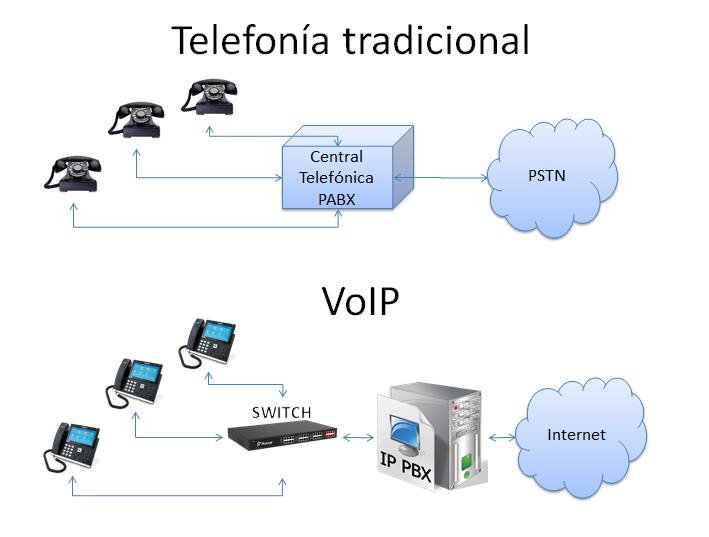
\includegraphics[width=\textwidth]{tradicionalVSvoip}
		
		%titulo de la imagen, salen debajo de la imagen y en el indice de imagenes.
		\caption{Telefonía tradicional versus VoIP}
		
		%centrado, por si las moscas
		\centering
		
		%para referencias
		\label{fig:ttvsv}
	\end{figure}

	Es muy importante diferenciar entre voz sobre IP (VoIP) y telefonía sobre IP 
	(ToIP) [Figura \ref{fig:ttvsv}]. Algunos autores \cite{switching} indican que 
	en forma general tanto VoIP como ToIP son términos intercambiables. Otros 
	\cite{voiptoip} definen a VoIP como el conjunto de normas, dispositivos, 
	protocolos que intervienen en la transmisión de voz sobre el protocolo IP, 
	conformando de esa forma una tecnología. Mientras que ToIP es el servicio 
	telefónico disponible al público basado en la tecnología VoIP, así como el conjunto de nuevas 
	funcionalidades que se ofrecen gracias al uso de la tecnología VoIP integrando 
	los servicios de datos y de voz, tanto analógica como digital. 
	
	En el presente documento se hará uso del término VoIP como la tecnología, 
	incluyendo los nuevos servicios integrados que se ofrecen gracias a esta 
	y el termino ToIP como el acto de simular aplicaciones de telefonía 
	tradicional a través del uso de VoIP.
	
	\begin{figure}[h]
		
		%nombre de la imagen, sin extencion. "width=\textwidth" ancho igual al texto
		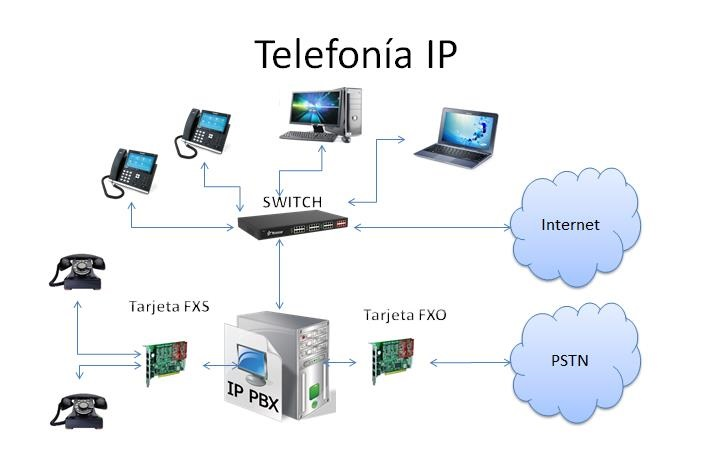
\includegraphics[width=\textwidth]{toip}
		
		%titulo de la imagen, salen debajo de la imagen y en el indice de imagenes.
		\caption{Esquema básico de Telefonía IP}
		
		%centrado, por si las moscas
		\centering
		
		%para referencias
		\label{fig:toip}
	\end{figure}

	
	
	

